%!TEX program = xelatex
\documentclass[zihao=-4,a4paper]{ctexart}
%==================== 数学符号公式 ============
\usepackage{xeCJK}
\newcommand{\zhongsong}{\CJKfontspec{STZhongsong}}%华文中宋,请自行下载字体并安装
\usepackage{fontspec}
\setmainfont{Times New Roman}

\usepackage{amsmath}                 % AMS LaTeX宏包
\usepackage[ruled]{algorithm2e}              %伪代码
%\usepackage{amssymb}                % 用来排版漂亮的数学公式
%\usepackage{amsbsy}
\usepackage[style=1]{mdframed}
\usepackage{amsthm}
\usepackage{amsfonts}
\usepackage{mathrsfs}                % 英文花体字 体
\usepackage{bm}                      % 数学公式中的黑斜体
\usepackage{bbding,manfnt}           % 一些图标,如 \dbend
\usepackage{lettrine}                % 首字下沉,命令\lettrine
\usepackage{gbt7714}                 %配置gb7714引用格式

\def\attention{\lettrine[lines=2,lraise=0,nindent=0em]{\large\textdbend\hspace{1mm}}{}}
\usepackage{longtable}
\usepackage[toc,page]{appendix}
\usepackage{geometry}                % 页边距调整
\geometry{top=2.5cm,bottom=2cm,left=2.5cm,right=2cm}
%\usepackage{relsize}                % 调整公式字体大小:\mathsmaller,\mathlarger
%\usepackage{caption2}               % 浮动图形和表格标题样式
\usepackage{booktabs}                %三线表上下加粗
\usepackage{diagbox}                 % 分类表头
%%%使用带圈数字作为教主
\usepackage{pifont}
\usepackage[symbol*,stable]{footmisc}
\DefineFNsymbols{circled}{{\ding{192}}{\ding{193}}{\ding{194}}
{\ding{195}}{\ding{196}}{\ding{197}}{\ding{198}}{\ding{199}}{\ding{200}}{\ding{201}}}
\setfnsymbol{circled}               %带圈脚注
%====================公式按章编号==========================
\numberwithin{equation}{section}
\numberwithin{table}{section}
\numberwithin{figure}{section}
%================= 基本格式预置 ===========================
\usepackage{fancyhdr}
\pagestyle{fancy}
\fancyhf{}  
\fancyhead[C]{\zihao{5}  \songti 英文论文翻译}
\fancyfoot[C]{~\zihao{5} \thepage~}
\renewcommand{\headrulewidth}{0.65pt} 
\ctexset{
    section = {
        format = \centering\bfseries\zihao{-2} \heiti,
        name = {第, 章}
    },
    subsection = {
        nameformat = \bfseries\zihao{3} \heiti
    },
    subsubsection = {
        nameformat = \bfseries\zihao{4} \heiti
    }
}
%================== 图形支持宏包 =========================
\usepackage{subfigure}
\usepackage{graphicx}                % 嵌入png图像
\usepackage{color,xcolor}            % 支持彩色文本、底色、文本框等
\usepackage{hyperref}                % 交叉引用
\usepackage{caption}
\usepackage{multirow}                  %合并表格
\usepackage{enumitem}
% set up labelformat and labelsep for figure
\captionsetup{labelsep=quad}
\captionsetup{figurewithin=section}

\renewcommand{\thesubfigure}{(\arabic{subfigure})} %还可设置图编号显示格式,加括号或者不加括号

%==================== 源码和流程图 =====================
\usepackage{listings}                % 粘贴源代码
\usepackage{tikz}                    
\usepackage{tikz-3dplot}
\usetikzlibrary{shapes,arrows,positioning}
%===================   正文开始    ===================
\begin{document}
%===================  定理类环境定义 ===================
\newtheorem{example}{例}              % 整体编号
%\newtheorem{algorithm}{算法}
\newtheorem{theorem}{定理}            % 按 section 编号
\newtheorem{definition}{定义}
\newtheorem{axiom}{公理}
\newtheorem{property}{性质}
\newtheorem{proposition}{命题}
\newtheorem{lemma}{引理}
\newtheorem{corollary}{推论}
\newtheorem{remark}{注解}
\newtheorem{condition}{条件}
\newtheorem{conclusion}{结论}
\newtheorem{assumption}{假设}
%==================重定义 ===================
\renewcommand{\contentsname}{目 ~~ 录}     
\renewcommand{\abstractname}{摘 ~~ 要} 
\renewcommand{\refname}{参考文献}     
\renewcommand{\indexname}{索引}
\renewcommand{\figurename}{图}
\renewcommand{\tablename}{表}
\renewcommand{\appendixname}{附录}
\renewcommand{\proofname}{证明}
\renewcommand{\algorithmcfname}{算法} 
%\renewcommand{\algorithm}{算法} 
%============== 封皮和前言 =================
%===============  封面  =================
\smallskip
\begin{center}

\vspace*{2.2cm}
\zhongsong{\zihao{1} 英文论文翻译} \\
\vspace*{3.3cm}
\heiti{\zihao{2} 基于 bim-建筑安全规划中的危害辨识及防范 }\\
\vspace*{5.5cm}

\zhongsong
\begin{tabular}{cc}
 \zihao{-2} 作者:&\underline{\makebox[7cm][c]{\zihao{-2}Sijie Zhang}} \\ 
 \\
 \zihao{-2}作者: & \underline{\makebox[7cm][c]{\zihao{-2}Kristiina Sulankivi}} \\ 
 \\
 \zihao{-2}作者: & \underline{\makebox[7cm][c]{\zihao{-2}Markku Kiviniemi}} \\ 
 \\
 \zihao{-2}作者: & \underline{\makebox[7cm][c]{\zihao{-2}Ilkka Romo}} \\ 
 \\
 \zihao{-2}作者: & \underline{\makebox[7cm][c]{\zihao{-2}Charles M. Eastman}} \\ 
 \\
 \zihao{-2}作者: & \underline{\makebox[7cm][c]{\zihao{-2}Jochen Teizer}} \\ 
 \\
\end{tabular} 
\end{center}

%%=============设计(论文)任务书===========
%\begin{center}
%\zihao{-2}\textbf{\songti 本科生毕业设计(论文)任务书} 
%\end{center}
%\smallskip
%\renewcommand{\arraystretch}{1.3}
%\begin{tabular}{lll}
%\zihao{4} \textbf{\songti 学生姓名: 曹宇} & & \zihao{4} \textbf{\songti 专业班级:\quad\quad 船海1006班} \\ 
%\zihao{4} \textbf{\songti 指导教师:徐海祥}&\makebox [3cm] & \zihao{4} \textbf{\songti 工作单位:\quad 武汉理工大学} \\ 
%\end{tabular}\\
%\begin{tabular}{lll}
%\zihao{4} \textbf{\songti 设计(论文)题目:}& \zihao{4} \textbf{\songti  武汉理工本科论文\LaTeX 模板 } &\\ 
%\zihao{4} \textbf{\songti 设计(论文)主要内容:} \\
%\end{tabular} \\ 
%\begin{enumerate}
%\item \LaTeX 环境的配置
%\item 主要字体的控制和数学公式的选用
%\item 图表和代码的粘贴
%\end{enumerate}
%\begin{tabular}{ll}
%\zihao{4} \textbf{\songti 要求完成的主要任务:}
%\end{tabular} \\ 
%\begin{enumerate}
%\item 选择合适的\TeX 编辑系统
%\item 学习如何使用控制代码完成排版
%\item 合理的安排学习和科研的时间来发展自己兴趣爱好
%\end{enumerate}
%\begin{tabular}{ll}
%\zihao{4} \textbf{\songti 必读参考资料:}
%\end{tabular}
%\begin{enumerate}
%\item \LaTeX  \quad User Manual
%\item  字体设计的艺术
%\end{enumerate}
%\begin{tabular}{lll}
%\zihao{4} \textbf{\songti 指导教师签名: }&\makebox [4cm]& \zihao{4} \textbf{\songti 系主任签名:} \\
%& & \zihao{4} \textbf{\songti 院长签名(章)}
%\end{tabular}
%\thispagestyle{empty}
%\clearpage
%%==========本科生毕业设计(论文)开题报告  =============
%\begin{center}
%\zihao{-2} \textbf{\songti 武汉理工大学}\\
%\zihao{-2} \textbf{\songti 本科生毕业设计(论文)开题报告} 
%\end{center}
%\begin{tabular}{|l|}
%\hline \rule[-2ex]{0pt}{5.5ex} \makebox[13.5cm][l]{\zihao{4} \heiti 1、目的及意义(含国内外的研究现状分析) } \\ 
%\quad \LaTeX 是国际通行的科技论文排版软件,国际上科研机构和大学都采用它写作\\
%\quad 国内著名高校都有自己的本科生\LaTeX 模板供毕业生使用\\
%\quad 但是武汉理工大学还没有本科生\LaTeX 模板可以参考\\
%\quad 人类的价值在于创造而不是索取 \\
%\hline \rule[-2ex]{0pt}{5.5ex}  \zihao{4} \heiti
%2、基本内容和技术方案\\ 
%\quad 采用GITHUB托管降低代码维护成本\\
%\quad 加入在线\TeX 编辑器的使用简介 \\
%\quad 授人以渔,注重方法和理念的引导\\
%\hline \rule[-2ex]{0pt}{5.5ex}  \zihao{4} \heiti
%3、进度安排 \\ 
%\quad 离 deadline 两个月吃喝玩乐 \\
%\quad 离 deadline 一个月吃喝玩乐 \\
%\quad 离 deadline 半个月吃喝玩乐 \\
%\quad 离 deadline 一个星期狂写论文 \\
%\hline \rule[-2ex]{0pt}{5.5ex} \zihao{4} \heiti
%4、指导教师意见 \\ 
%\quad 曹宇同学是个好同志\\
%\quad 曹宇同志是个好同学\\
%\quad 本表格是支持跨页的长表格,你可以复制上面的内容进行测试\\
%\quad 具体方法是将tabular改为 longtable然后再编译\\
%\makebox[10cm][r]指导教师签名:\\
%\makebox[12cm][r]\quad 年\quad 月\quad 日\\
%\hline 
%\end{tabular} 
%\thispagestyle{empty}

\pagestyle{plain}
\pagenumbering{Roman}
\section*{\zihao{-2} \centering 摘 ~~ 要}

\vskip0.5cm
建筑信息模型在建筑设计和建筑规划中的应用正在迅速发展。基于 BIM 的建模和 4D 仿真(3D 和调度)为安全和物流
应用带来了许多好处。然而,到目前为止,在建模和规划安全过程方面只开发了有限的自动化。本研究的目的是探
讨如何在建筑项目的规划阶段的早期识别和消除潜在的跌落危险,这些危险是不知不觉地纳入施工进度表的。

本文首
先介绍了国内外建筑安全与 BIM 的研究概况。然后,提出了一个包含 BIM 安全规则自动检查算法的框架。开发的原
型使用模型进行了测试,其中包括芬兰的一个办公室和一个住宅建筑项目。第一个案例研究突出了手动与自动交配
的安全建模跌倒保护系统的比较。它还描述了保护安全设备模型的多种设计和建成方案的细节。第二个案例研究展
示了将该框架应用于项目进度计划的结果。它特别模拟跌落危险的检测和预防。这项工作的贡献是一个自动化的规
则检查框架,有效地将安全融入 BIM,并为从业人员提供一种检测和预防跌落相关危险的方法。会上还讨论了有关
已开发的先进型产品商业化的公开问题,并探讨了扩大传统安全管理做法对解决实地安全问题可能产生的影响。


{\zihao{4} \heiti 关键词: } \zihao{-4}建筑信息模型,建筑安全规则和代码检查,防止坠落危险,通过设计进行计划、调度和模拟预防
\addcontentsline{toc}{section}{摘要}

\clearpage
\section*{\zihao{-2} \centering \textbf{Abstract} }
   %用了Times New Roman字体来美化观感

   The applications of Building Information Modeling (BIM) in building design and construction planning
   are growing rapidly. BIM-based modeling and 4D simulation (3D and schedule) has brought many
   benefits to safety and logistics applications as well. However, only limited automation in modeling
   and planning safety processes has been exploited so far. The objective of this study is to investigate
   how potential fall hazards that are unknowingly built into the construction schedule can be identified
   and eliminated early in the planning phase of a construction project. A survey of research on construction
   safety and BIM is presented first. Then, a framework was developed that includes automated safety rule-
   checking algorithms for BIM. The developed prototype was tested using models including an office and a
   residential building project in Finland. The first case study highlights the comparison of manual vs. auto-
   mated safety modeling of fall protective systems. It also describes the details to multiple design and as-
   built scenarios where protective safety equipment is modeled. The second case study presents results of
   applying the framework to the project schedule. It specifically simulates fall hazard detection and pre-
   vention. The contribution of this work is an automated rule-checking framework that integrates safety
   into BIM effectively and provides practitioners with a method for detecting and preventing fall-related
   hazards. Presented are also discussions of open issues regarding commercialization of the developed pro-
   totype and considerations which explore what impact it might have on resolving safety issues in the field
   by extending traditional safety management practices.

\textbf{\zihao{4} Key Words:} Building Information Modeling,Construction safety rule and code checking,Fall hazard prevention,Planning;scheduling;and simulation,Prevention through Design
\addcontentsline{toc}{section}{Abstract}





\pagestyle{empty}
\tableofcontents 
\thispagestyle{empty}
%============== 论文正文   =================
\pagestyle{fancy}
\pagenumbering{arabic}
\section{介绍}
工作场所伤害、疾病和死亡统计数据表明,建筑施工中的职业健康
和安全 (OHS) 仍然是一个全球性问题。超过三分之一 (36\%) 的美国工作场
所的死亡事故发生在建筑业。同样,芬兰的建筑业造成了四分之一的死
亡职业事故。与其他几个行业一样,安全规划在生产规划领域占有关键地
位。然而,在建筑施工行业的安全,安全规划是与工程项目设计及规划阶段分开进行。
尽管高处坠落仍然是建筑工地的一个主要安全风险。但是在大
多数现有项目中,高处坠落保护计划通常要等到施工开始后才会制定。在施
工计划阶段发现和解决安全问题时还会出现其他问题。例如,在建筑工
程项目存在的恶劣天气(气候、独特性)和动态(多种资源、时间限制)条件
下,工人层面的安全交流尤其具有挑战性。以前的几项研究也报告了类似
的问题。

有效的安全规划的主要障碍之一是传统的安全规划仍然主要依赖
纸质的二维图纸和时间表来了解建筑工地的安全装备需求。在防止高处坠落
方面,图 \ref{fig:c1f1} 提出了一个传统的防跌落计划的例子,其中各种防跌落系统已被
标记为不同颜色的建设计划

\begin{figure}[thbp!]
    \centering
    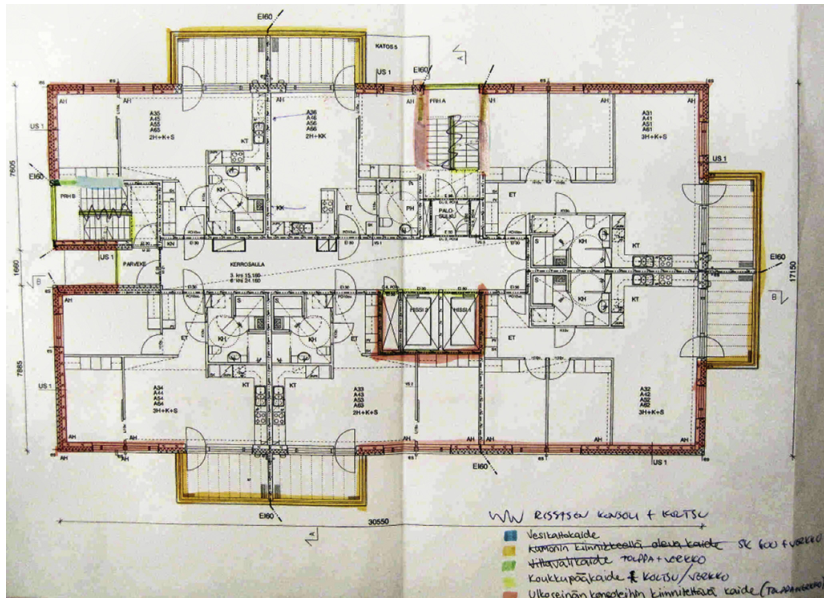
\includegraphics[width=0.8\linewidth]{res/c1f1.png}
    \caption{传统跌落保护计划的示例}
    \label{fig:c1f1}
    \end{figure}

这样手工的高处坠落危害辨识和计划会导致低效率,其中一些原因是:

\begin{itemize}
    \item 它需要专业的安全工程师根据自己的经验发现潜在的安全隐患并确定安全设备。
    \item 许多安全问题是隐含的,因为建筑计划中没有标明部分完整的条件。
    \item 建设项目的动态性导致了安全需求的变化。基于静态图纸,很难确定不同施工阶段、进度表的潜在跌落危险。
    \item 施工进度会因天气、材料交付等因素而发生变化,导致安全计划发生变化。每次更改时间表都要更新安全计划,这既费时又费力。
    \item 举例来说,与小的孔洞能给足部造成伤害相比,人会更容易发现他们自己即将在边缘跌落到低处。这些漏洞很难或从未在纸质计划中绘制,因此可能永远不会被发现,即使是专家。
\end{itemize}   

目前用于处理和报告建筑项目安全和健康相关问题的方法效率低下。
新型技术可以协助施工安全专家更容易识别和解决安全隐患,同时解决施工现
场条件的复杂性和动态性,从而可以更安全的施工和更少的努力。

建筑信息模型 (BIM) 是一种对设备的物理和功能特性的数字表示建筑
信息模型。BIM 是一种共享的知识资源,用于获取有关设施的信息,这
些信息为设施在其生命周期中的决策提供了可靠的基础;定义为从最初构
想到拆除的存在。建筑信息模型 (BIM) 在建筑/工程/建筑 (AEC) 和设施
管理 (FM) 行业的不断推广,正在改变人们对待安全的方式。建筑信息
模型 (BIM) 在施工作业计划和管理以及安全管理中的应用正在迅速增加。
一个出发点是在建筑设计和工程阶段的早期强调安全方面。 Zhang et al 同时指出,
建筑业需要解决目前使用的纸张和人工安全程序效率低下的问题。

基于 BIM 的方法正被应用于建筑设计和规划。在工地安全管理和监
督方面也越来越多地实施这些措施。人工安全检查通常遵循以下程
序:
\begin{itemize}
    \item 使用建造工程进度表,以确定建造工程的施工动作、次序或工程任务项目的空间布局
    \item 确定造成安全隐患的临时条件
    \item 规划纠正措施以消除安全隐患
    \item 将这些纠正措施整合到方案中
\end{itemize}

然而,人类的认知技能仅限于心理模拟。
复杂的环境表明,一个更加积极的、基于仿真的方法和使用预定义的模式检查
可以大大加强这一系列活动的有效性。
正如 Kiviniemi 所说,只有拥有一套完整的方法才能成功地提供所有领域的能力。

在前人研究成果的基础上,本研究旨在开发一个基于 BIM 的跌落危
险自动识别与规划工具,该工具

\begin{itemize}
    \item 基于施工进度动态识别潜在跌落危险
    \item 有效协助劳动密集型作业的防跌落系统的建模与规划任务
    \item 通过可视化潜在危险提高工人的安全意识
\end{itemize}

本案例研究还旨在评估自动化安全代码检
查和规划的可能性、好处和开发需求。此外,我们还研究了开发的基于
BIM 的原型工具的可用性和成熟性,该工具用于支持建筑施工项目中的
预防规划。

本文结构如下:第一部分对传统的减灾方法和信息建模在施工安全规
划中的应用进行了综述。第二部分介绍了已开发的安全规则检验原型及
其计算方法。第三部分介绍了原型在两个案例研究中的应用。在第一个案例
研究中,讨论了跌落保护系统的人工建模和自动建模,并对设计方案与
实际情况进行了比较。在第二个案例中,以施工进度计划为例,说明了
样机产生的跌落危险检测和防护的动态特性。第四部分比较了几种 BIM 在
建筑安全规划中的应用。论文的最后一部分对研究结果和贡献进行了总
结和讨论。      %
\section{背景}
\subsection{传统的风险分析和减轻灾害}
Hinze 等人调查了使用历史信息的有效性。例如,他审查了职业安全与健
康管理局(OSHA)可记录的伤害率,以提高建筑项目的安全绩效。
利用历史信息的一个有价值的替代方法是使用领先的安全性能预测指标,作为未来安全性能水平预测指标的措施
安全指标或安全风险分析是预防建筑安全事故发生的关键环节。发展「建造业工作安全分析」,
以识别潜在的失控事件及评估事件发生的机会。
Shapira 根据塔式起重机的运作
情况,制订了一套全面的安全水平指标。与考虑在一般建筑场地上使用
塔式起重机不同,他增加了一个因素,针对特定场地的个性化安全水平。
Hallowell 和 Gambatese 建立了混凝土模板施工安全风险等级量化方法。
尽管研究集中在积极利用技术提高安全风险水平上,但是迄今为止还没有实用的方法来解
决如何将这些数据用于工业从业人员和 BIM 技术之中。因此,开发更先进的方法
来整合这些信息就显得尤为重要。

\subsection{施工安全规划中的信息建模}
新兴技术包括数据库、计算机辅助模拟和可视化技术为安全规划提供了新的机
遇。其中许多起源于传统的安全研究。例如
Hinze、Gibb、Choudhry、Toole 、Gambatese、Lingard 和 Wakefield 等人
通过设计 (PtD) 在建筑业的操作安全和健康 (OHSC) 的方式为预防工作贡献了基础研究。
这些研究成果激励了其他研究人员,甚至更先进的方法,开发或应用新兴技
术到 OHSC。

Hadikusumo 和 Rowlinson 开发了一个安全过程设计(DFSP)工具,以帮助用户识别建筑构件和
过程中固有的安全隐患。DFSP 数据库包含建筑物目标、相关潜在安全隐
患和可能的事故预防数据库。它引入一套综合安全及建造管理系统,使用
现有的四维计算机辅助设计模型。发展概念框架采用虚拟原型技术,以
协助建造业的安全管理。它由三个部分组成:建模与模拟、不安全因素的
识别和安全培训。探讨了可视化技术在地铁施工安全管理和风险评估中
的应用。然而,随着施工进度的提高,行业也需要探索更先进、更有效的方法
来实现安全危害辨识和可视化。

BIM 已经被迅速认识到它可以改变建筑项目交付的过程。也认识到
BIM 可以用来促进安全管理,并与其他施工计划过程相结合。 Turner 建筑
公司建立了一个标准化的模型检查程序,以确保他们的项目符合严格的安全
标准。他们的 BIM 专家开发了一个基于 Solibri 模型检查器 (SMC) 的规
则集包。芬兰的 VTT 技术研究中心已经开发了一个详细的防坠落建模
和 4D 可视化框架。工作内容包括临时安全构筑物和进行安全施工所需
设备的建模。它还为建筑物中安全设备的永久安装建立模型,用于建造、
运行和维护阶段。人们还尝试展开最佳实践,以改善承建商、设计师和
分包商之间的协作规划程序。这些现有的研究无疑为使用 BIM 改进安全
规划和危害辨识铺平了道路,而与手动过程相比,需要更智能的方法来
提供自动化和时效性方式的安全规则检查。

将安全管理任务连接到 4d 模型中,为审查和评估作为施工操作一部
分的安全提供了全新的机会。例如,它可以加强安全规划方面的合作,
增强整体安全沟通。4D 规划可以创建一个安全规划实践,这个实践在
一个项目中比在传统的建筑项目中开始得更早。此外,它可以产生更详
细的安全规划。例如,早期的安全计划,可能需要。
与防跌落相关的建模包括护栏、保护罩和网以及安全带锚点的安全特征构成 4D 模型。
Zhou 提出了一种基于 4D 建设规划的协作方法。他们提出建筑安全及数码设计的新研
究方向,例如利用技术让建筑工人与设计师分享知识,以及利用视觉化
技术将建筑地盘的知识融入设计。 Zhang 开发了一个基于 BIM 的自动化工具,
可以帮助检测潜在的坠落危险,包括从前面板边缘、板孔和墙壁开口处
坠落。

除了自动的安全检查,还有能力自动建模建议的跌倒防护,这可以是一
个劳动密集度很大的任务,当使用现有的 BIM 为基础的软件,自动规则检
查的工业基础类 (IFC) 的模式,也已经得到了研究。
然而,到年开发框架的可能性和目前的限制还不清楚。需要努力研究在
现有的施工规划流程中实施这种原型的适用性、局限性和要求。

4D 方法的一个重大缺陷是依赖于计算机化的施工进度表。施工作业
是动态的,可能会发生与原计划工程不符的变更。因此,数码时间表很
少经常更新,以准确反映在任何特定时间点正在进行的所有行动。同时,
建议安全建模与永久安装的建筑部件的设计和工程相同水平的细节,
这使得计划和模型维护工作更加复杂。在这种基于 BIM 的规划活动中,
需要额外的安全知识、时间和技术资源,使实际执行变得困难。因此,
在大规模应用于该领域之前,对于从业人员来说,了解额外的建模要求
和基于 BIM 的安全危险检测和预防工具的好处是有益的。
\section{基于 BIM 的规则检查}
\subsection{规则检查方法}
现有的安全规则、指南和最佳实践可以与现有的三维 (3D) 设计和进度
信息结合使用,以形成一个自动化的安全规则检查系统。其目的是在建
筑物建造时自动识别这些动态条件,在虚拟 3D 空间中识别它们的位置,
并交互式或自动地为多种危险提供解决方案和保护系统的可视
化。

这个平台可以作为一种工具,使人们能够方便地、易于理解地
看到随着时间的推移在建筑和安全方面取得的最新进展,特别是能够发
现工地上的危险地点。安全措施的指示将有助于安全管理人员在施工计
划阶段以及施工期间提前规划安全。规则检查程序包括以下程序:

\begin{itemize}
    \item 规则解释:从安全规则或最佳实践(例如,OSHA)对安全规则的解
    释是一个基于逻辑的映射,从人类语言到机器可读的形式。可
    以从书面规则中分析和提取规则中的名称、类型和其他属性。
    构建模型准备:必须很好地构建构建模型,以包括用于进行规则
    检查的所需对象、属性和关系。此外,由于防堕设备的需要取
    决于施工工作的状况,因此需要一个包括建筑组件安装时间表/
    顺序的 4D模型。
    \item 规则执行:规则执行阶段将转换后的规则集与准备好的构建模型
    集合在一起。该规则可应用于数以千计的条件情形,需要组合
    跟踪。规则的执行有两个步骤:(a)自动检查模型以识别不安全的
    条件,(b)识别和应用候选解决方案
    \item 纠正不安全情况的行动。这最后一步可以通过多种方式控制,
    对每种情况进行人工干预,通过应用规则来确定最佳修正,从
    而完全自动地解决问题。
    \item 规则检查报告:检查结果可以以多种形式报告:(a)使模型中应用的
    安全防护设备可视化,(b)基于 excel的不安全状况报告和采取的
    纠正措施。此外,为安全设备的资源平衡和将生成的信息导入
    项目进度表提供数量启动信息也是可能的。
    \item 安全纠正:在建筑工地上采取的主要纠正措施是根据规则检查报
    告安排和跟踪(安全)材料的后勤运输。例如,一个现场的实现可
    以是在 BIM 平台上报告,该平台为建筑楼层安装和拆除安全设
    备分配工作任务。
    \item 这是对规则检查系统()一般需求的扩展,包括了安全改进步骤。
\end{itemize}

\subsection{基于规则的算法在案例研究中的应用}

一旦建立了良好的建筑物信息模型,并且建立了模型对象与调度之
间的联系,就可以应用规则进行安全隐患的检测。 Zhang 给出了如下的解释方法:

\begin{enumerate}
    \item 板坯边缘保护:图 \ref{fig:c3f1} 解释了根据 OSHA 安全规则检测所需预防方法的算法
    对于每个任务,它检查 slab 对象是否链接到给定的工作任务。对
    于与任务相关联的每个 slab 对象,该算法检查 slab 是否需要与现
    有的 slab 合并。如果在同一水平面上没有现有的板,则计算板边
    界。此外,现有的墙壁膨胀检测,看看是否有任何部分的板边界
    不需要下降保护。因此,无保护的边缘需要护栏保护计算。另外,
    根据平板合并后的几何条件分别计算存在边、未保护边和重叠边。
    因此,新的护栏安装没有保护的边缘和现有的护栏重叠的边缘被
    删除。
    \item 板坯孔保护:一般有两种方法检测板坯孔洞:基于几何的检测和基于对象的检测。由于某些孔洞
    是设计人员为建立复杂的板几何模型而切割的,因此不应将其归
    类为潜在落差孔洞。因此,即使基于几何的检测可以找到所有的
    内部多边形的板,这些将包括一些假阳性错误。对于基于对象的
    检测,它需要额外的标记努力,以协助从模型中的其他空洞对象
    的孔识别。在这项研究中,我们主要依靠基于物体的目标识别,
    但也通过比较板的深度和孔的深度来检查是否是一个会产生坠落
    危险的直通孔。理想情况下,为了清楚地区分这两种情况,在建
    模阶段,工程师应该有两种不同的工具/按钮来(a)为复杂几何和
    (b)为实际切割平板而切割。
    \item 墙体开孔保护:墙体开孔检测过程类似于板坯孔检测。要考虑的特殊
    情况是墙元件的位置:它是内墙还是外墙。对于那些位于板的边缘
    的,一旦墙元素已经安装完毕后,可以拆除板坯边缘保护的护栏,同时,如果存在墙
    口需要进行保护。如果在靠近内墙的地方没有板孔(例如电梯井的
    孔),则不需要考虑或保护墙开口。
\end{enumerate}

\begin{figure}[thbp!]
    \centering
    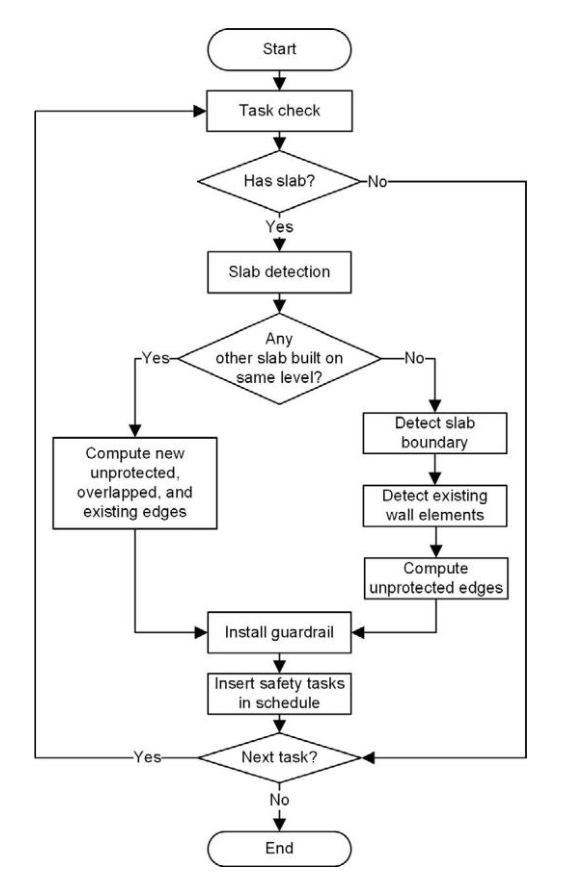
\includegraphics[width=1.0\linewidth]{res/c3f1.png}
    \caption{检测板坯边缘所需预防措施的规则检查算法}
    \label{fig:c3f1}
\end{figure}





\section{基于 BIM 的跌落危险检测和\\预防规划案例研究的经验教训}
\subsection{案例研究 1:手工建模与自动建模的比较}

在第一个案例研究中,对办公楼地下室现浇混凝土的防坠落设备进
行了人工和自动建模。比较了两种方法的优缺点。\\

(1)安全防护装备的手工模型:\\

为了了解安全预防系统建模和计划编制工作的复杂性,图 \ref{fig:c4f1} 首先在 BIM
中进行了人工建模和计划编制。展示了一张照片和模型化的 3d 安全栏
杆组件,因为它通常用于芬兰的建筑项目。所选择的护栏解决方案为领
先的边缘板表面包括护栏的职位和木材栏杆。定制安全部件的 3D 表示
是手工建模的。现实的护栏解决方案是基于最佳实践信息承包商提供并
在建筑工地使用。职位的几何对应的芬兰 Vepe 产品。扶手、中间护栏
和脚趾板的尺寸与现有规格相符。

\begin{figure}[thbp!]
    \centering
    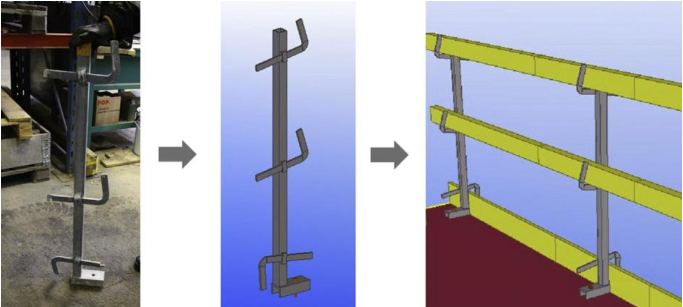
\includegraphics[width=1.0\linewidth]{res/c4f1.png}
    \caption{工程安全护栏设备模型(表面安装护栏柱与木质护栏一起使用)}
    \label{fig:c4f1}
\end{figure}

其想法是在板边缘规划护栏柱的位置,以便在施工期间无需移动护栏柱。
这样既可节省时间,又可减低从高处堕下的风险。如果
栏杆靠近混凝土柱(见图 \ref{fig:c4f2}),栏杆柱与设计柱之间有一定距离。
在钢梁上有预制孔的前缘使用相同的安全栏杆解决方案,确保安全设备的快速安装和拆卸(见图 \ref{fig:c4f3})

\begin{figure}[thbp!]
    \centering
    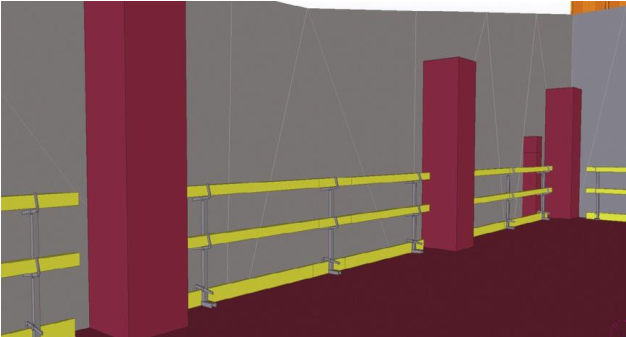
\includegraphics[width=1.0\linewidth]{res/c4f2.png}
    \caption{基于 BIM 的防坠计划:现浇板边缘的安全栏杆)}
    \label{fig:c4f2}
\end{figure}

\begin{figure}[thbp!]
    \centering
    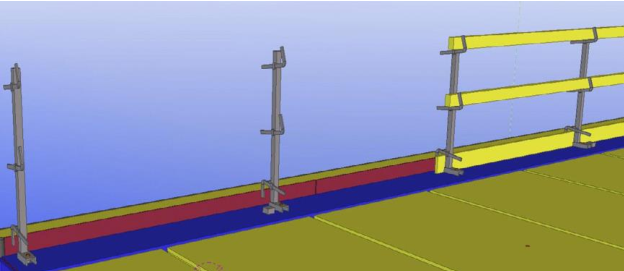
\includegraphics[width=1.0\linewidth]{res/c4f3.png}
    \caption{同样的安全栏杆解决方案模拟到上层办公楼:护栏柱安装在预制钢梁的预先设计孔中)}
    \label{fig:c4f3}
\end{figure}

手动生成的基于BIM的安全护栏平面图连同一些模型视图一起交付给承包商,
这些模型视图提供了在现场实施的模型化解决方案。
由于临时安全设备的 4D 调度与当前的BIM建模工具复杂,
VTT 研究团队将混凝土和钢框架施工相关的防坠落可视化,
并将永久性建筑结构和任何临时安全设备的工作流程计划和可视化。

在实际试验开始之前,对项目中的 4D BIM 工具的使用进行了功能测试。
测试项目是一个办公楼,最初是由该项目的结构工程师使用 Tekla Structures 软件建模。
结果表明,交互式4D坠落防护规划,特别是安全栏杆的调度和可视化,为实际工作者提供了一种可行的方法。

从实际出发,为了实现基于4D BIM的临时结构规划和可视化,
需要对其建模和可视化进行一些特殊的要求或设置。
例如,在4D模拟方面,临时结构在不再需要后需要从模型中移除或者是隐藏。\\

(2)基于规则检测算法的跌落危险自动检测与防护\\

人工建模的坠落防护方法提供了对施工现场潜在坠落危险的良好理解,通常具有较高的详细程度。
但是,由于手动建模的耗时性,建议使用自动建模方法。本文提出的系统已在同一试点工程中得到应用。
图 \ref{fig:c4f4} 展示了开发的系统在地下室一层的自动建模结果。\\

\begin{figure}[thbp!]
    \centering
    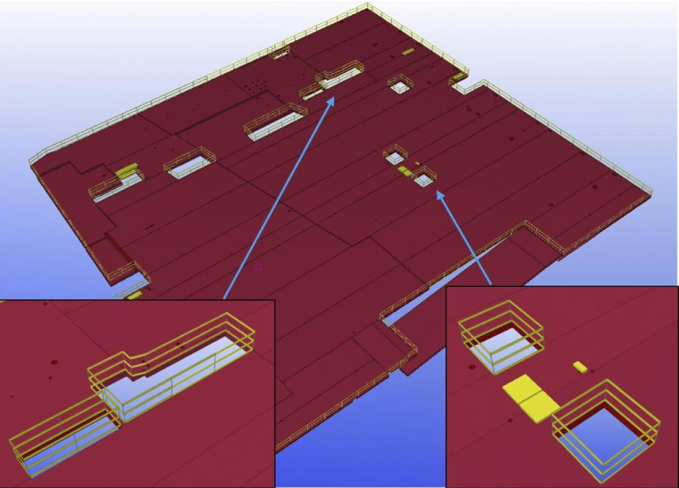
\includegraphics[width=1.0\linewidth]{res/c4f4.png}
    \caption{板边孔自动检测及护栏安装效果}
    \label{fig:c4f4}
\end{figure}


(3)基于手动 BIM 跌落保护方法建模经验\\

通过建立同一办公楼结构模型中的安全栏杆和楼盖模型,进行了跌
落危险的检测和防范规划。这种规划比传统的人工规划更为详细。

现场工作人员指导研究组实施的规划和建模。该规划和建模工作比工作阶段的开始早了三个月。
在目前的规划实践中,此类详细的防坠落规划并没有在项目阶段的早期进行。
只选择和采购所需的安全设备类型,并提出了更全面的防坠落安排计划。

图 \ref{fig:c4f5} (a-j) 展示了如何在BIM和施工现场实施基于模型的防坠落计划。
由于视角稍有不同,图片之间存在一些视觉差异。一些图片还展示了混凝土模板的模型。
当它影响到安全栏杆的位置时,它的各个部分的建模要比安全栏杆更抽象。

\begin{figure}[thbp!]
    \centering
    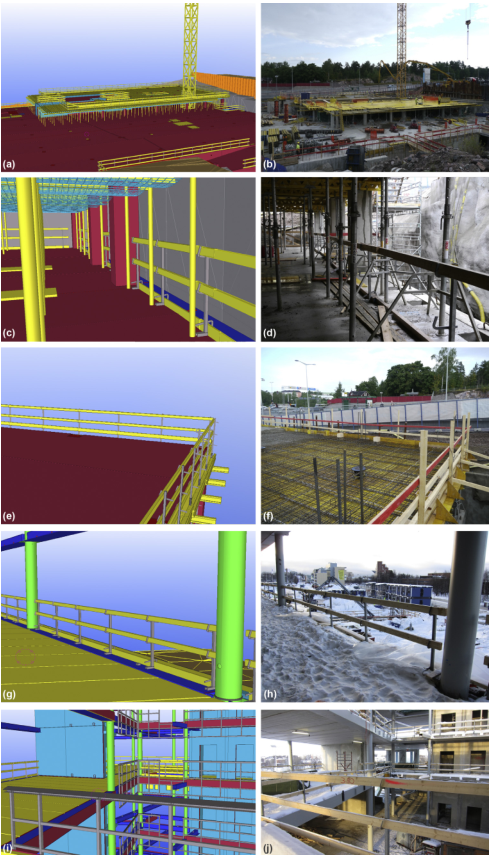
\includegraphics[width=0.8\linewidth]{res/c4f5.png}
    \caption{比较模型和现场情况:a,b 为地下室施工阶段试验现场的一般视图;c,d 是板前缘;e,f为混凝土板模板;g,h是安全轨柱用螺栓连接到钢梁上的焊接螺纹套筒,以及 i,j 为办公楼的中庭临时防坠落系统的一般视图)}
    \label{fig:c4f5}
\end{figure}

目前的一个区别是,材料、设备和其他暂时性的构造对象并没有在 BIM 中建模。
然而,由于这些对象可能是事件的参与者或导致事件发生,因此也应该对它们进行建模。
分析行业的详细工作活动和空间需求可能是有用的,因为行业在本质上是高度动态的。
这些问题都不在本文的讨论范围之内。

板边缘安全栏杆的位置与平面图相比发生了实质性的变化(见 图 \ref{fig:c4f5} c 和 d)。
计划位置的最初想法是允许在靠近边缘的栏杆后面安装墙构件。
在现场安全栏杆的实施阶段,决策者决定将护栏进一步放置在板内,以便栏杆形成连续的护栏。

临时楼梯是地下室较低楼层的紧急出口,如图 \ref{fig:c4f6} 所示。
由于脚手架建模需要其他工具,因此在建模时未计划设置护栏。改变安全栏杆位置的一个主要原因是占地面积需要三条腿支撑架的空间。
一旦护栏向内移动,中间的栏杆必须拆除。另一个原因可能是,
规划期间使用的最新 BIM 版本的结构模型确实包含了几个用于将立面元素固定到楼板边缘的方孔。

\begin{figure}[thbp!]
    \centering
    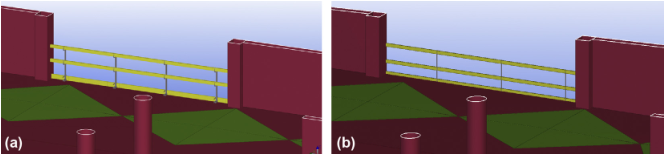
\includegraphics[width=1.0\linewidth]{res/c4f6.png}
    \caption{(a) 手动与(b)自动建模结果}
    \label{fig:c4f6}
\end{figure}

这些孔限制了护栏安装的可用区域。此外,由于安全规划是在施工前三个月完成的,
因此最近的变更可能不会在 BIM 中实施。因此,使用 BIM 的详细安全隐患检测和预防计划应始终接近施工,
并使用最新和最新版本的 BIM。基于 BIM 的详细安全规划还应与所有项目干系人,
特别是最终负责安全设备实施的分包商进行协调。其他风险可能与使用其他工具类似。
管理人员应当把建模结果作为最终确认的结果,当建模结果提示为危险时应该完全信任他;
现场应该使用软件测算的结果来管理,应该避免管理者使用他们自己的的技能和经验。

在许多项目中,设计方案和施工方案也可能不同。混凝土板前缘的安全栏杆(见\ref{fig:c4f5} e 和 f)在设计方案上是金属柱和木制护栏。
然而,在现场施工则使用了一种使用木桩作为临时的解决方案。
如果不遵守标准,偏差就可能会导致严重的安全问题。这种偏差和材料更换需要现场人员解释情况。
在现场使用人造安全设备当然不遵循安全规定,除非是为了克服不可预见的现场条
件。
图 \ref{fig:c4f5} 的 g 和 h 显示了试点项目的一个上层的安全栏杆,它使用了一种栏杆的解决方案——
即用螺栓将立柱连接到钢梁的螺纹套筒上。这些固定件焊接到钢制车间的钢梁上。
它们已经出现在钢框架的结构模型中,套筒为栏杆柱提供了一种快速可靠的固定方法。
选定的工艺有利于安全安装和拆除安全栏杆,特别是在恶劣的现场条件(即天气)下。


试点大楼的内部有一个中庭空间,每一层都需要防坠落装置。设计
的 BIM 模型建议在钢结构安装完毕后立即安装最终的护栏系统。这可以
通过在吊装到位之前将护栏预先焊接到钢材上来实现。
然而,最初设计
的解决方案并没有在年实施由于护栏类型的改变而造成的场地。承建商不得不对这一变化迅速做出
反应,并在施工期间实施了传统的护栏系统,后来被永久护栏系统所取
代(见图 \ref{fig:c4f5} i 和 j)。设置临时护栏系统的另一个常见原因是为了避免在施工过
程中损坏固定的永久护栏。在这两种情况下,规则检查系统都可以有效
地生成解决方案。\\

(1) 人工与自动落地保护模型建立方法的比较\\

自动建模方法的优点如下(见表\ref{tb:compare}):(1)使用自动建模方法所需的时间比手
动建模大大减少。对于像案例研究项目这样复杂的建筑模型,通常需要
几秒或几分钟才能生成结果。
手动建模需要更高的安全专业知识和建模熟悉程度。建模人员需要充分
理解模型,知道如何添加和调度栏杆组件,更重要的是,建模人员需要
熟悉安全规则和需求。然而,安全专门知识并不是自动化方法的必要先
决条件,因为已知边界已经存储在系统中并编入程序。(3)一旦进行了设
计变更或进度更新,手工更新相应的安全要求是困难和耗时的。相反,
自动安全检查系统可以很容易地重新启动以生成新的结果。(4)手动建模
可以提供更高层次的细节的安全解决方案(见)。在施工柱和墙体之前,
板边护栏需要拆除。在(a)项中,栏杆柱被小心地安置在靠近柱子的位置,
这样以后就不需要额外的柱子了。然而,自动化建模并没有考虑这些细
节。在(b)中,在柱和墙的结构完成后,需要在靠近左侧柱的地方增加一
个柱子。针对护栏无法延伸一定距离,必须自动设立立柱的问题,提出
了一种解决方法。

\begin{table}[thbp]
    \caption{手工和自动建模方法的比较}
    \begin{center}
        \begin{tabular}{@{}lcc@{}}
            \toprule
            \multicolumn{1}{c}{\textbf{}} & \textbf{手工建模} & \textbf{自动建模} \\ \midrule
            \textbf{时间需求} & 长 & 短 \\
            \textbf{安全知识需求} & 非常多 & 少 \\
            \textbf{更新困难性} & 困难 & 简单 \\
            \textbf{细节的等级} & 高 & 低 \\ \bottomrule
            \end{tabular}
    \end{center}
    \label{tb:compare}
    \end{table}

\subsection{案例研究 2:BIM 中的动态跌落危险检测和预防}

在第二个案例研究中,开发的自动规则检查工具应用于多层预制公寓建筑模型(见图 \ref{fig:c4f7})。
目标是根据项目进度动态演示安全检查结果。所有预制混凝土构件均已制造并运至施工现场,
并将按照预先确定的顺序从 A 部分开始安装,然后是 B 部分和 C 部分。预制混凝土就位后,
在现场建造外墙保温层和砖墙。该项目的结构模型已使用 Tekla Structures 17.0 建模软件进行建模。
开发的自动规则检查平台所需的4D进度表是根据从承包商获得的信息添加到结构模型中的。
该信息由现场工程师以施工进度表和涉及安装顺序的工作分解结构(WBS)的传统格式提供。

\begin{figure}[thbp!]
    \centering
    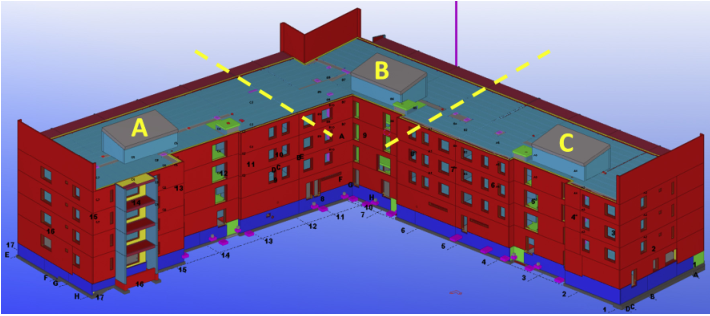
\includegraphics[width=1\linewidth]{res/c4f7.png}
    \caption{多层预制公寓建筑模型及其剖面图}
    \label{fig:c4f7}
\end{figure}


图 \ref{fig:c4f8} 可以近距离观察到混凝土板块。在楼板安装完毕之后,对楼板的连
接部分进行加固和浇筑,而在下一层楼板安装之前,墙板安装已经开始。
墙体和升降机井与楼板一起作为一个结构系统工作,将荷载传递到基础
上。楼板部分是按层安装的。一个截面的一层楼大约需要7天的时间,
一个截面的搭建大约需要 5-6 周的时间。护栏解决方案需要根据板截面的增长进行更新,
例如,当两个板截面在同一水平面上合并时,需要移除中间的护栏。

\begin{figure}[thbp!]
    \centering
    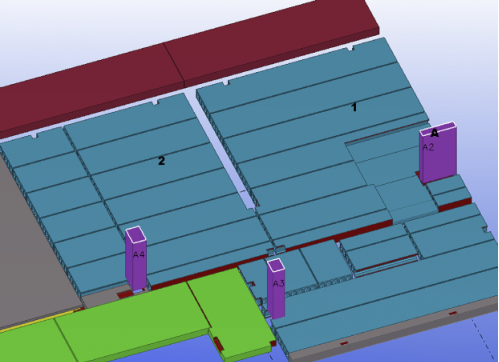
\includegraphics[width=0.8\linewidth]{res/c4f8.png}
    \caption{预制板面板近景}
    \label{fig:c4f8}
\end{figure}
\newpage
在完成规则检查算法的基础上,它实现了包括护栏在内的防坠落系统
的自动可视化。

它还为在施工进度中安装和拆除安全相关设备创建了子任务。并
将其纳入施工进度表。
图 \ref{fig:c4f9} 示出了部分更新的具有所需安全解决方案的时间表。
图 \ref{fig:c4f10}示出了模型模拟的四个不同阶段,
可以实现安全设备嵌入模型和施工进度的时间可视化。
4D模拟的对象表示如图 \ref{fig:c4f11} 所示。一楼的楼板从 A 段到 B 段,
由于施工过程中有时会合流,中间的护栏必须拆除,
拆除也改善了现场的工作流程,因为工人现在可以安全地从A段走到B段而不必绕道。
建筑顺序的安装和拆除如图 \ref{fig:c4f12}(a)和(b)所示。

\begin{figure}[thbp!]
    \centering
    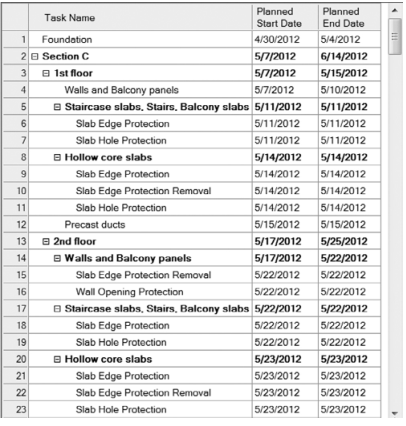
\includegraphics[width=0.8\linewidth]{res/c4f9.png}
    \caption{更新的包括防坠落方法的安装和拆除的施工进度表}
    \label{fig:c4f9}
\end{figure}

\begin{figure}[thbp!]
    \centering
    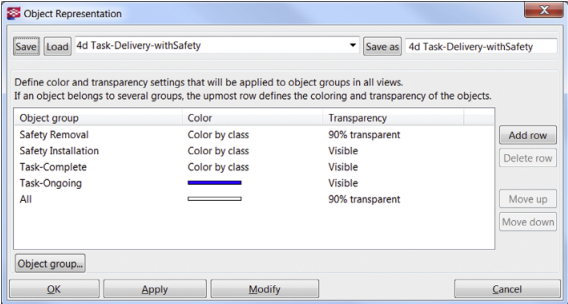
\includegraphics[width=0.8\linewidth]{res/c4f10.png}
    \caption{4D 模拟的对象表示设置}
    \label{fig:c4f10}
\end{figure}

\begin{figure}[thbp!]
    \centering
    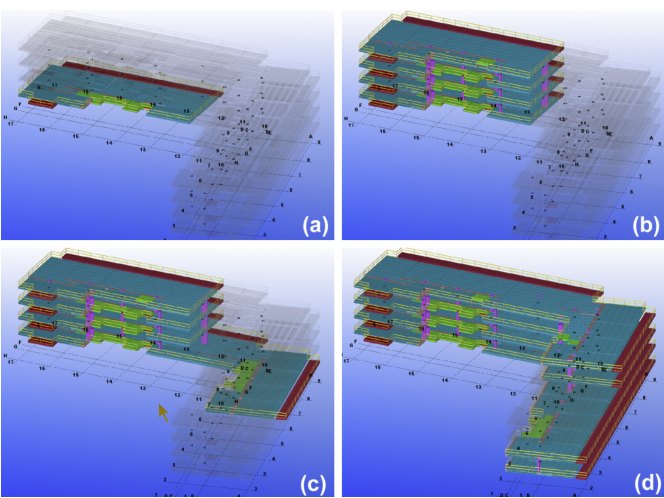
\includegraphics[width=0.8\linewidth]{res/c4f11.png}
    \caption{模型板、柱和护栏防护系统的4D仿真}
    \label{fig:c4f11}
\end{figure}
\newpage
\begin{figure}[thbp!]
    \centering
    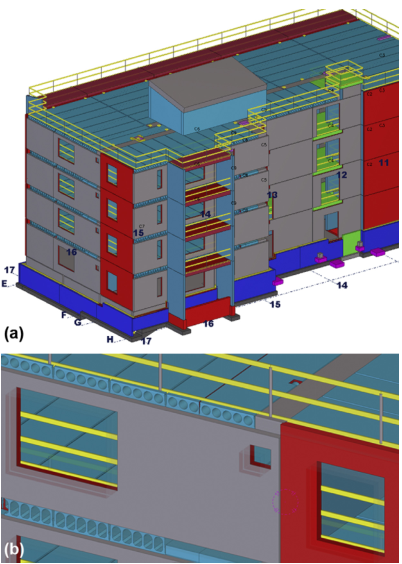
\includegraphics[width=1\linewidth]{res/c4f12.png}
    \caption{(a) 建筑物 a 区的防坠落保护系统和(b)墙洞保护的近景}
    \label{fig:c4f12}
\end{figure}

图 \ref{fig:c4f12} 示出了板边缘保护和墙洞口保护的更详细视图。在模型中生成安全防护系统后,
也会自动生成检查报告。然后,可以将该报告导出为 MS-Excel 格式,如 图 \ref{fig:c4f13} 所示。
这种文件格式允许现场安全或监督人员简化生成数据的使用。
例如,他们可以计算保护工作场所所需的安全设备。
最终,该清单还可能支持详细安全解决方案的预制,这些解决方案可以在场外预制,
并以与定制预制混凝土板类似的方式安装。
因此,开发的工具及其生成的数据支持多种安全设计 (Design-for-Safety,DfS) 概念。
该清单也可用作检查清单,以确保所有必需的安全防护系统已在施工现场到位。

板坯开孔检查的用户界面如图 \ref{fig:c4f14} 所示。用户可以使用工具的界面根据不同的预防方法定义自己的需求。
规则执行后,安全防护设备将在模型中可视化,检查结果将在单独的对话框中列出,
安全管理人员可以从中预览结果,并在必要时手动进行更改。
这使得人类决策者随时处于安全防护危险检测和预防的循环中。

\begin{figure}[thbp!]
    \centering
    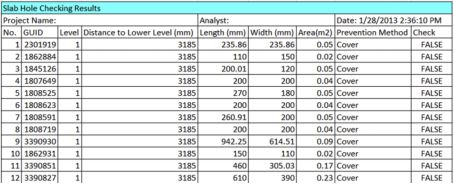
\includegraphics[width=1\linewidth]{res/c4f13.png}
    \caption{材料清单:板孔检查结果为安全设备的估算和预制提供了Excel表}
    \label{fig:c4f13}
\end{figure}

\begin{figure}[thbp!]
    \centering
    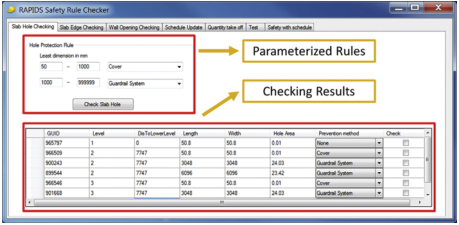
\includegraphics[width=1\linewidth]{res/c4f14.png}
    \caption{板孔检查的用户界面}
    \label{fig:c4f14}
\end{figure}

\newpage
\subsection{讨论}

该工具能够自动、成功地检测出无防护板边缘并安装护栏系统。利
用 BIM 软件的内置功能,可以方便地计算护栏的起吊量。此外,自动安
装的板边缘和窗口护栏可以由用户手动修改。

在试验过程中,工具中成功地集成了所谓钩柱的详细三维模型(见图17)。
用户现在可以为安全扶手建模选择简化的模型表示或详细的表示(自定义构件)。
此外,更详细的护栏模型和相关的安全设备零部件,如焊接配件,
可以自动添加到钢梁或混凝土面板中进行护栏安装建模。
在钢梁或混凝土面板的制作中可以预先考虑相应的连接,从而减少高空作业。
然而,如果用户的目标是提供详细和自动化的安全建模,
那么还需要进一步开发一个程序来改进岗位规则。

目前开发的系统的一个限制是它严重依赖于 BIM 提供的信息,如几何结构和时间表。
如果BIM中的信息不完整、不正确或不准确,安全分析的正确性将受到很大影响。
此外,建筑模型几何结构(例如,具有复杂空间相关性的对象形状)或场地条件
(例如,有助于施工过程且通常未建模的临时结构)可能导致当前版本的规则检查系统的应用失败,
或者最多产生经验丰富的安全专家能够理解和解决的结果。为了获得更准确的结果,
建议首先运行自动系统来对照模型进行检查


目前开发的系统的一个局限性是,它严重依赖 BIM 提供的信息,如
几何图形和时间表。如果 BIM 中的信息不完整、不正确或不准确,安全
分析的正确性将受到很大影响。此外,构建模型的几何形状(例如,具有
复杂空间依赖性的对象形状)或场地条件(例如,有助于构建过程且通常
未建模的节奏元结构)可能会导致规则检查系统当前版本的应用失败,或
者产生经验丰富的安全专家能够理解和解决的最好结果。为了获得准确
的结果,建议先运行自动化系统对照模型进行检查。
安全专家随后会审核结果,并提供意见。目前,Zhang 等人使用开发的原型工具会
自动创建概念性防坠落计划。未来研究的另一个领域是生成工艺流程图,以及安全工程师、专家和检查员的作用,
因为他们应该充分利用基于BIM的安全隐患探测预防规划工具。朝着这一方向迈出的第一步是自动化
工作危害分析(JHA)。\\

根据已进行的测试结果,今后可能需要改进的地方包括:

\begin{enumerate}
    \item 为安全元素提供高层次的细节:例如,例如,护栏的柱子和板子可以通过带
    有抽象线条的 BIM 可视化。
    经验不足的用户可能更喜欢高层次的视觉细节以及它看起来像什么,比如如果需要锚定,
    这些位置需要被确定。有经验的用户可能对附加功能的高层次细节感兴趣,
    例如,当某些安全设备可以预制时。了解护栏柱与建筑构件之间的复杂连接可以加快此类构件在现场的安装过程。
    \item 使用独立于软件的数据交换格式:独立于软件的数据交换格式便于多个项目涉众之间的通信。
    出于安全规划的目的,需要探索一种基于IFC 的解决方案。
    使用 IFC 模型进行自动安全检查和规划的能力将使在
    各种 BIM 模型创作工具中创建的模型具有更广泛的检查能力。
    \item 在复杂模型测试:未来,更全面的基于BIM的防坠落规划解决方案需要在复杂模型几何结构上进行测试,
    并提供全系列安全解决方案的高水平细节。例如,在施工期间以及设施运行和维护期间,
    安装备用解决方案,如安全网和挂钩。
\end{enumerate}
\section{审查 BIM 平台以支持安全规划}
\subsection{已知问题}
对一些商业化 BIM 平台的支持安全规划的能力进行了检查。若干功
能性先决条件被认为对于启用基于 bim 的安全规划非常重要。它们的名
单如下:

\begin{enumerate}
    \item 调度和模拟:建筑业的复杂和动态特性及其现场工作模式已经被广泛的认同。
    为了在施工过程中发现和预防安全隐患,需要将工程进度与
    BIM 联系起来。此外,如何根据施工进度计划进行施工进度的可
    视化,提高施工人员的安全意识和沟通能力是施工进度计划可视
    化的关键。    
    \item 建模:建筑安全不仅是管理或控制工人的安全行为,还包括设计、采
    购、安装和拆除安全和节奏设备,如护栏、脚手架和安全网或挂
    钩。为了可视化和定量化的目的,在 BIM 中对这些临时对象进行
    设计和建模是非常必要的。因此,一个理想的平台需要能够创建和修改模型项,并提供可视化。
    \item 施工现场布置建模与可视化:认识施工现场物流的重要性和施工现场
    的动态性,从安全角度考虑施工现场布置的重要性。现场布局的
    建模和可视化能力可以支持详细、准确的现场逻辑分析,从而提
    高生产率和工作场所安全性。
    \item 模型格式:如前所述,使用 IFC 数据 for-mat 允许对各种 BIM 创作工具
    中包含的模型进行更一般的检查。
    \item 规则检查能力:BIM 平台配备了自己的规则引擎,可以为用户提供自
    定义或用户配置的规则检查过程安全规则的机会。
\end{enumerate}


几个现有的商业化 BIM 软件解决方案的比较及其结合安全的潜力见表 \ref{tb:CP}

\begin{table}[thbp]
    \caption{四种 BIM 应用的比较分析}
    \begin{center}
        \begin{tabular}{@{}lcccccc@{}}
            \toprule
            \multicolumn{1}{c}{\multirow{2}{*}{\textbf{应用软件}}} & \multicolumn{6}{c}{\textbf{功能}} \\ \cmidrule(l){2-7} 
            \multicolumn{1}{c}{} & \textbf{计划} & \textbf{模拟} & \textbf{主体建模} & \textbf{施工平面图建模} & \textbf{基于 IFC 格式} & \textbf{规则检查} \\ \midrule
            \textbf{Autodesk Revit} & - & - & √ & √ & - & - \\
            \textbf{Autodesk Navisworks} & √ & √ & - & - & - & - \\
            \textbf{Solibri Model Checker} & - & - & - & - & √ & √ \\
            \textbf{Tekla Structures} & √ & √ & √ & - & - & - \\ \bottomrule
            \end{tabular}
    \end{center}
    \label{tb:CP}
\end{table}
\newpage
SMC 作为一种基于 BIM 的工具的优势在于它能够使用 IFC 数据交换
格式,这使得基于 BIM 的建模软件的检查工作可以成为一种独立的工具来使用。规则检
查功能和用户界面还提供了合并安全解决方案的可能。然而,尽管自
动化被用来进行日常的检查工作,仍然需要人工对所有与安全相关的临
时设备和结构进行建模,这些设备和结构在基于 BIM 的建模软件中现有
的对象库中有的不被支持,有的缺乏项目。根据项目的规模或复杂程度,冗长的模型修
改过程通常需要几天甚至几周的时间。在 Navisworks 上也发现了类似的
问题,由于缺乏建模功能,很难添加与安全相关的设备。施工现场的动
态特性无论是在施工现场管理系统中还是在施工现场管理系统中都无法
体现出来,这使得施工现场管理系统在不同的施工阶段都需要进行规范
检查。由于本文侧重于建筑物相关的跌落危险,场地布局建模和可视化
不属于本文研究的范围。因此,在比较分析的基础上,选择 Tekla Structures
作为本文研究的安全规则检测算法的实现平台。另外,为了使建筑信息
模型能够应用于施工过程规划或分析,需要进行大量的现场布局和操作
建模工作。
\section{总结}
开发的建筑物信息模型跌落危险检测与预防安全规则检查平台已在
两个案例中成功实现。该算法能够检测混凝土板和前缘中潜在的坠落危
险的位置,并提供相应的坠落防护装置的安装指南(例如,材料清单、可
视化),实际上解决了 BIM 中确定的坠落危险。结果表明,该方法在安
全设计和规划阶段能够有效地探测和可视化潜在的跌落危险。

由于自动生成的防坠落计划必须由安全专家检查,但如果遵循其他安全指南或有更好地实践方法,
也允许进行调整。开发的平台显示出强大的潜力,可以创建基于 BIM 的安全计划,
可视化施工进度表中的安全性,安排安装和拆除工作,
并提供包括永久性建筑部件和临时安全设备在内的选项和程序,并模拟它们。

未来的一个目标可能导致安全行业最佳做法的重大变化,即基于 
BIM 的安全规划可能成为标准建筑物建设规划过程的一部分。基于 BIM 
的建模还可以增加安全理解和交流,尤其是在工程设计和施工计划阶段。
由于建筑信息模型中的施工进度表与模型对象之间只有几个星期的时间,
因此在施工对象的结构模型、施工进度表或原始安装顺序发生变化之后,
有必要检查模型是否发生了变化,并更新检查结果。开发的系统通过消
除设计和规划阶段的危险,确保采购安全设备,并在需要时在正确的地
点和时间准备好安装,协助人类决策制定者进行这一审查过程。

在考虑基于 BIM 的安全规划自动化取代人工建模的优点时,发现通
过减少时间和人工建模工作,自动化有可能显著提高基于 BIM 的计划编
制过程。一旦发生设计变更,就需要使用手动建模进行额外的工作。需
要时间和其他人力资源仔细检查模型,以确保模型护栏或其他防护设备
仍然有效和准确。虽然人工建模的优点是人类参与了每一步,但是它很
耗时,而且可能容易出错。一个系统,提供自动化和一致的结果,然后
由一个人审查,可以提供更频繁和更快的更新。

目前对所开发系统应用的关注包括:(1)以模型为基础的设计和施工图
纸在动态的施工环境中经常发生变化,因此有必要定期检查模型,以确保
安全状况识别和纠正措施是最新的;(2)自动安全模型的质量和详细程度
可能需要进一步发展,以满足设计部门和建筑工地从业员的实际需要,
并非所有模型都能提供安全规划及检查所需的资料,例如墙体与平板部
分之间的关系(例如连接)可能未能妥善建立或正确建模。这可能会防止
识别拆除护栏的建设进展。这种与安全相关的设计标准或者延伸的 BIM
要求需要被研究和正式化。
%============= 参考文献 =====================
\addcontentsline{toc}{section}{参考文献}
{\zihao{5} \songti \bibliography{bibfile}}
\clearpage
\newpage
\appendix

%=============  致谢  ======================
\section*{致 ~~ 谢}
\addcontentsline{toc}{section}{致谢}
本报告中介绍的结果是基于 RAPIDS 建筑安全技术实验室、芬兰
VTT 技术研究中心、芬兰斯堪斯卡公司和 Tekla 公司的合作。这项研究
由芬兰研究项目 BIMCON(工业化建筑供应链中基于信息模型的产品数
据管理)资助,该项目是芬兰研究项目 PRE的一部分。是由 RYM 有限公
司和芬兰研究机构、大学和公司联合组织的。资金由 Tekes(芬兰技术和
创新基金机构)提供。项目由芬兰 Skanska 公司协调,其他项目参与方包
括芬兰 VTT 技术研究中心、ParmaOy、WeberOyAb、RautaruukkiOyj、
TeklaOyj 和阿尔托大学。
\end{document}
%%%%%%%%%% 结束 %%%%%%%%%%
